\chapter{Experimental Results and Discussion}{}{}
\label{CH:EXP}%




%==================== Section =====================%
\section{Dataset}
\label{sec:dataset}

The proposed framework is trained and evaluated on standard 
video super-resolution benchmarks under bicubic downsampling 
with a scale factor of $\times 4$ (BIx4 degradation). Four 
publicly available datasets are used: REDS, Vid4, UDM10, and 
SPMCS. These datasets cover diverse content and motion 
characteristics, allowing the evaluation to assess both 
in-domain performance and cross-dataset generalization.


\subsection{Dataset division}
\label{subsec:dataset_division}

The four datasets are partitioned into training and evaluation 
roles as summarized in Table~\ref{tab:dataset_division}. The 
REDS dataset is used for training, while four datasets are used 
for evaluation: REDS4 as the in-domain evaluation set, and Vid4, 
UDM10, and SPMCS as cross-dataset evaluation sets.

\begin{table}
\centering
\caption{Dataset division for training and evaluation.}
\label{tab:dataset_division}
\resizebox{\textwidth}{!}{
\begin{tabular}{|l|l|c|c|}
\hline
Dataset & Role & Sequences & Resolution \\
\hline\hline
REDS (train split) & Training & 240 & 720p \\
\hline
REDS4 & In-domain evaluation & 4 & 720p \\
Vid4 & Cross-dataset evaluation & 4 & SD \\
UDM10 & Cross-dataset evaluation & 10 & 720p \\
SPMCS & Cross-dataset evaluation & 30 & SD \\
\hline
\end{tabular}
}
\end{table}

\textbf{Training set.} The REalistic and Dynamic Scenes (REDS) 
dataset \cite{nah2019reds} was originally introduced for the 
NTIRE 2019 video super-resolution challenge. The full dataset 
contains 270 high-quality video sequences captured at 720p 
resolution, each consisting of 100 consecutive frames at 24 
frames per second. The dataset is characterized by diverse 
motion patterns and rich content variations, including human 
activities, vehicle motion, and natural scenes, making it 
suitable for training generalizable VSR models. The dataset is 
officially split into 240 sequences for training, 30 for 
validation, and 30 for testing. Following the standard 
convention established in BasicVSR \cite{chan2021basicvsr} and 
adopted by subsequent diffusion-based VSR works including 
StableVSR \cite{rota2024stablevsr}, the proposed framework is 
trained on the 240 training sequences.

\textbf{In-domain evaluation set.} Within the REDS training 
split, four sequences (clip indices 000, 011, 015, and 020) are 
reserved for evaluation as REDS4. This subset has become the de 
facto in-domain benchmark for VSR methods trained on REDS, 
providing a controlled evaluation setting where the test 
distribution matches the training distribution.

\textbf{Cross-dataset evaluation sets.} Three additional 
benchmarks are used to assess generalization to unseen content 
distributions:

\begin{itemize}
    \item Vid4 \cite{liu2013vid4} consists of four short 
    sequences (calendar, city, foliage, walk) with diverse 
    content characteristics: textual textures, urban structures, 
    non-rigid natural motion, and articulated human motion. 
    Despite its compact size, Vid4 is widely adopted as a 
    standard cross-dataset benchmark.
    \item UDM10 \cite{yi2019udm10} contains 10 high-quality 720p 
    sequences with relatively static content and high-frequency 
    textural detail. The high-quality ground truth makes UDM10 
    particularly suitable for evaluating fine-detail restoration.
    \item SPMCS \cite{tao2017spmcs} consists of 30 sequences spanning diverse outdoor activities, natural phenomena, and 
    motion patterns. Among the four evaluation sets, SPMCS has 
    the most content diversity, providing the most challenging 
    cross-dataset evaluation.
\end{itemize}


\subsection{Dataset Construction}
\label{subsec:dataset_construction}

To learn the perceptual and temporal characteristics of video 
content effectively, we construct the training and evaluation 
data following the standard protocol established in BasicVSR 
\cite{chan2021basicvsr} and adopted by subsequent diffusion-
based VSR works including StableVSR \cite{rota2024stablevsr}. 
The high-resolution (HR) frames are provided directly from the 
source datasets, while the low-resolution (LR) frames are 
generated via bicubic downsampling with an anti-aliasing filter:
\begin{equation}
    I^{LR} = \mathcal{D}_{\mathrm{bicubic}}(I^{HR}; s=4),
    \label{eq:bicubic_degradation}
\end{equation}
where $\mathcal{D}_{\mathrm{bicubic}}$ denotes bicubic 
downsampling with an anti-aliasing filter and $s=4$ is the 
downsampling scale factor (BIx4 degradation). For REDS, this 
produces LR frames at $180 \times 320$ from HR frames at 
$720 \times 1280$.

In the training process, we follow the temporal window strategy 
adopted by StableVSR \cite{rota2024stablevsr}, where each 
training sample consists of a 3-frame temporal window 
$\{I^{LR}_{t-1}, I^{LR}_t, I^{LR}_{t+1}\}$ centered at frame 
$t$, paired with the HR ground-truth frame $I^{HR}_t$. 
According to Rota \emph{et al.}, this 3-frame window provides 
sufficient temporal context for the conditioning branch to 
estimate optical flow between adjacent frames while keeping 
memory consumption manageable for diffusion-based training 
\cite{rota2024stablevsr}.

We trained a specific number of frames (\textit{nframes}) per 
sequence on the REDS dataset, where the frames are randomly 
selected from each 100-frame sequence to form one training 
sample. Rota \emph{et al.} use the entire 100 frames per 
sequence with a temporal window of 3 frames during StableVSR 
training, while we adopt a similar window-based sampling 
strategy. To match the iteration budget reported in StableVSR 
(20K iterations) and conform to fair comparison settings, we 
allocated \textit{nframes} as 100 for REDS, with random spatial 
crops of size $64 \times 64$ extracted from the LR frames 
(corresponding to $256 \times 256$ HR patches) and random 
horizontal flipping applied as data augmentation. The 3-frame 
window is preserved across the augmentation to maintain 
temporal coherence within each sample.

Table~\ref{tab:nframes} shows the frame sampling and batch 
construction for one training step comparing with the StableVSR 
baseline \cite{rota2024stablevsr}. The total 
$(N_{\mathrm{batch}} \times T_{\mathrm{window}}) \times C$ 
frames were used during training, where $N_{\mathrm{batch}}$ is 
the batch size, $T_{\mathrm{window}}$ is the temporal window 
size (3 frames), and $C=3$ represents the RGB color channels. 
Therefore, $(8 \times 3) \times 3 = 72$ frames are processed in 
one training step. The number ``8'' represents the batch size, 
``3'' represents the temporal window (previous, current, next 
frames), and the second ``3'' represents the RGB color channels.

\begin{table}[htbp]
\caption{Frame sampling and batch construction for one training 
step.}
\label{tab:nframes}
\centering
\resizebox{\textwidth}{!}{
\begin{tabular}{|c|l|c|c|c|c|c|}
\hline
& Dataset & nframes & 
$(N_{\mathrm{batch}}, T_{\mathrm{window}})$ & 
LR patch size & HR patch size & Total frames/step \\ 
\hline\hline
StableVSR* & REDS & 100 & (8, 3) & $64 \times 64$ & $256 \times 256$ & 24 \\ 
\hline\hline
& Dataset & nframes & 
$(N_{\mathrm{batch}}, T_{\mathrm{window}}) \times C$ & 
LR patch size & HR patch size & Total frames/step \\ 
\hline\hline
Ours & REDS & 100 & $(8, 3) \times 3$ & $64 \times 64$ & $256 \times 256$ & 72 \\ 
\hline
\end{tabular}}
\end{table}

In addition to the HR-LR frame pairs, our framework requires 
the four-level DT-CWT decomposition of each LR frame to 
construct the frequency-domain conditioning. The DT-CWT 
coefficients are computed on-the-fly during training using the 
\texttt{pytorch\_wavelets} library \cite{cotter2019pytorch}, 
producing the magnitude tensor $M^{(j)}$ (18 channels per 
scale) and the trigonometric phase encoding 
$\mathcal{T}(\phi^{(j)}) = (\sin\phi^{(j)}, \cos\phi^{(j)})$ 
(36 channels per scale) for $j \in \{1, 2, 3, 4\}$.

For evaluation, full-resolution LR frames are processed without 
spatial cropping. Each frame is super-resolved using a sliding 
3-frame window centered on the target frame; for boundary 
frames at the start and end of each sequence, the window is 
symmetrically padded by duplicating the boundary frame. All 
evaluations are conducted in the RGB color space using a unified 
evaluation script to ensure metric consistency across the 
compared methods.

Furthermore, in order to compare our model with other models 
fairly and conform to the standard VSR evaluation setting, we 
have guaranteed the values of \textit{nframes}, batch size, and 
temporal window are consistent across the StableVSR baseline 
and our proposed method on the same dataset. The only 
configuration that differs between the two methods is the 
addition of the four-level DT-CWT decomposition computed from 
the same LR frames, which constitutes the unique technical 
contribution of this work.


%==================== Section =====================%
\section{Training Details}
\label{sec:training_details}

All models were trained using the PyTorch deep learning 
framework with the diffusers library 
\cite{vonplaten2022diffusers} for the diffusion pipeline, and 
used single GPU for training. Table~\ref{tab:environment} shows 
the specifications of the experimental environment.

\begin{table}[htbp]
\caption{Environment condition for experiments.}
\centering
\begin{tabular}{c|c}
\hline
ITEMS & spec \\
\hline\hline
OS      & Ubuntu 20.04 LTS \\
CPU     & Intel Xeon \\
GPU     & NVIDIA RTX 3090 (24GB) \\
Mem     & 128GB \\
Framework & PyTorch 2.0 / diffusers \\
\hline
\end{tabular}
\label{tab:environment}
\end{table}

In all experiments, we used the AdamW optimizer 
\cite{kingma2014adam} with $\beta_1=0.9, \beta_2=0.999$ and 
initial learning rate $1 \times 10^{-4}$ that remains constant 
throughout training. The proposed framework is built upon the 
StableVSR pipeline \cite{rota2024stablevsr}, which adapts 
Stable Diffusion v2.1 \cite{rombach2022ldm} for video 
super-resolution. The pre-trained U-Net (472.4M parameters) 
and VAE (55.3M parameters) from Stable Diffusion v2.1 are kept 
frozen throughout training to preserve their generative prior. 
The ControlNet branch (207.7M parameters) is jointly fine-tuned 
alongside the proposed Frequency Encoder, which contributes 
6.22M trainable parameters. To assess the generalization 
performance of the proposed Frequency Encoder, no pre-trained 
weights are used; it is trained from scratch using the 
identity-preserving initialization, where the SFT heads are 
initialized to produce $\gamma \equiv 1$ and $\beta \equiv 0$ 
at step 0, ensuring that the wrapped U-Net behaves identically 
to the original at the start of training and gradually learns 
meaningful frequency-domain modulation throughout the 20{,}000 
training iterations.

The Dual-Tree Complex Wavelet Transform is implemented using 
the \texttt{pytorch\_wavelets} library 
\cite{cotter2019pytorch} with \texttt{biort=`near\_sym\_a'}, 
\texttt{qshift=`qshift\_a'}, and $J=4$ decomposition levels. 
The four scales are partitioned into the high-frequency band 
$\mathcal{H} = \{j=1, j=2\}$ injected at \texttt{up\_blocks[1]} 
of the U-Net decoder, and the low-frequency band 
$\mathcal{L} = \{j=3, j=4\}$ injected at 
\texttt{down\_blocks[1]} of the U-Net encoder.

The high-frequency, low-frequency, and lowpass loss weights 
are set to $\lambda_{\mathcal{H}} = 0.1$, 
$\lambda_{\mathcal{L}} = 1.0$, $\lambda_{\mathrm{LP}} = 1.0$, 
following the design intent described in 
Section~\ref{subsec:wavelet_loss}: the high-frequency band 
serves as a soft texture prior requiring only a small relative 
weight, while the low-frequency and lowpass components require 
strong supervision for structural reconstruction. A 
sensitivity analysis on these weight ratios is presented in 
Section~\ref{subsec:ablation_loss_weights}.

The wavelet loss is applied every $K=4$ optimization steps as 
a practical compromise to limit the VAE-decoding overhead 
while still providing regular frequency-domain supervision 
throughout the 20{,}000 training iterations.

For diffusion-based training, the proposed framework is 
trained for 20{,}000 iterations on the REDS training split. 
Each training sample consists of a 3-frame temporal window 
with random spatial crops of size $64 \times 64$, batch size 
of 8, and random horizontal flipping as data augmentation. 
At inference time, 50 DDPM denoising steps are used following 
the StableVSR protocol with bidirectional sampling, where the 
diffusion process alternates between forward and backward 
temporal directions across denoising steps to enhance temporal 
consistency.


%==================== Section =====================%
\section{Evaluation Metrics}
\label{sec:metrics}

A comprehensive evaluation in video super-resolution requires 
metrics that capture multiple, often competing, aspects of 
quality. Pixel-level fidelity metrics measure how closely the 
predicted frame matches the ground truth but correlate poorly 
with human perception, particularly for generative models that 
synthesize plausible but non-pixel-accurate details. Perceptual 
metrics address this gap by leveraging deep features or 
human-aligned quality models. Temporal metrics, unique to 
video tasks, assess inter-frame consistency. To provide a 
complete picture, the proposed framework is evaluated using 
nine metrics spanning four categories: reconstruction fidelity, 
full-reference perceptual quality, no-reference perceptual 
quality, and temporal consistency.


\subsection{Reconstruction Fidelity Metrics}
\label{subsec:fidelity_metrics}

\textbf{Peak Signal-to-Noise Ratio (PSNR)} measures pixel-level 
fidelity between the super-resolved output and the ground-truth 
high-resolution frame. PSNR is defined as
\begin{equation}
    \mathrm{PSNR} = 10 \log_{10} 
    \left( \frac{\mathrm{MAX}^2}{\mathrm{MSE}} \right),
    \label{eq:psnr}
\end{equation}
where $\mathrm{MAX}$ is the maximum possible pixel value (255 
for 8-bit images) and $\mathrm{MSE}$ is the mean squared error 
between the predicted and ground-truth frames. Higher PSNR 
values indicate better pixel-level fidelity. However, PSNR 
correlates poorly with human perception and tends to penalize 
generative models that synthesize realistic textures with 
non-identical pixel values.

\textbf{Structural Similarity Index Measure (SSIM)} 
\cite{wang2004ssim} compares local luminance, contrast, and 
structural patterns between the predicted and ground-truth 
frames. SSIM is more aligned with human visual perception than 
PSNR but still prioritizes structural fidelity over perceptual 
realism, often favoring over-smoothed outputs.


\subsection{Full-Reference Perceptual Metrics}
\label{subsec:fr_metrics}

\textbf{Learned Perceptual Image Patch Similarity (LPIPS)} 
\cite{zhang2018lpips} measures perceptual similarity using 
deep features from a pre-trained network. LPIPS computes the 
weighted $L_2$ distance between feature activations across 
multiple network layers, with weights learned to match human 
perceptual judgments. Lower LPIPS values indicate better 
perceptual similarity.

\textbf{Deep Image Structure and Texture Similarity (DISTS)} 
\cite{ding2020dists} extends perceptual similarity by 
explicitly combining structure and texture similarity through 
deep features. Unlike LPIPS, DISTS is robust to texture 
variations: visually similar but pixel-different textures are 
considered similar by DISTS. This property makes DISTS 
particularly suitable for evaluating restoration methods that 
synthesize plausible textures.


\subsection{No-Reference Perceptual Metrics}
\label{subsec:nr_metrics}

No-reference (NR) metrics assess perceptual quality without 
requiring a ground-truth reference. This category is 
particularly important for evaluating generative models, as 
full-reference metrics may unfairly penalize realistic outputs 
that deviate from pixel-level ground truth. Three complementary 
NR metrics covering different paradigms are used.

\textbf{Multi-scale Image Quality Transformer (MUSIQ)} 
\cite{ke2021musiq} is a deep learning-based metric using a 
transformer architecture trained on large-scale 
human-annotated quality ratings. MUSIQ processes images at 
multiple scales to capture both local details and global 
appearance, outputting a score from $0$ to $100$, with higher 
values indicating better perceptual quality.

\textbf{Contrastive Language-Image Pre-training Image Quality 
Assessment (CLIP-IQA)} \cite{wang2023clipiqa} leverages the 
pre-trained CLIP model \cite{radford2021clip} to assess 
quality through vision-language alignment. CLIP-IQA computes 
the similarity between the input image and quality-related 
text prompts (e.g., ``a good photo'' versus ``a bad photo''), 
producing a score in $[0, 1]$ that captures high-level semantic 
quality.

\textbf{Natural Image Quality Evaluator (NIQE)} 
\cite{mittal2013niqe} is a classical NR metric based on natural 
scene statistics. NIQE measures the deviation between the 
statistical features of the input image and a multivariate 
Gaussian model fitted to natural images. Lower NIQE values 
indicate that the image's statistics more closely match those 
of natural images. Unlike MUSIQ and CLIP-IQA, NIQE is fully 
unsupervised, requiring no human quality ratings.

These three metrics provide complementary perspectives on 
perceptual quality: MUSIQ captures human-aligned quality, 
CLIP-IQA captures semantic naturalness, and NIQE captures 
statistical naturalness.


\subsection{Temporal Consistency Metrics}
\label{subsec:temporal_metrics}

Temporal consistency is a critical aspect of video 
super-resolution. A method producing high-quality individual 
frames but lacking temporal coherence will exhibit flickering, 
severely degrading perceived video quality.

\textbf{Temporal LPIPS (tLPIPS)} \cite{chu2020temporal} 
measures perceptual differences between consecutive frames:
\begin{equation}
    \mathrm{tLPIPS} = \frac{1}{T-1} \sum_{t=1}^{T-1} 
    \mathrm{LPIPS}(\hat{I}_t, \hat{I}_{t+1}),
    \label{eq:tlpips}
\end{equation}
where $\hat{I}_t$ is the $t$-th generated frame. Lower tLPIPS 
indicates higher temporal consistency. tLPIPS is particularly 
effective for diffusion-based VSR evaluation, as it captures 
texture-level flickering that pixel-level metrics miss.

\textbf{Temporal Optical Flow (tOF)} \cite{chu2020temporal} 
measures motion consistency by comparing optical flow fields 
between the generated and ground-truth videos:
\begin{equation}
    \mathrm{tOF} = \frac{1}{T-1} \sum_{t=1}^{T-1} 
    \big\| \mathrm{Flow}(\hat{I}_t, \hat{I}_{t+1}) 
    - \mathrm{Flow}(I_t, I_{t+1}) \big\|_1.
    \label{eq:tof}
\end{equation}
Lower tOF indicates better preservation of motion patterns. 
While tOF and tLPIPS both assess temporal consistency, they 
capture complementary aspects: tOF measures motion fidelity, 
while tLPIPS measures perceptual texture consistency.

%==================== Section =====================%

\section{Performance Analysis}
\label{sec:performance_analysis}

The performance is evaluated using nine quantitative metrics 
spanning four categories: reconstruction fidelity (PSNR, SSIM), 
full-reference perceptual quality (LPIPS, DISTS), no-reference 
perceptual quality (MUSIQ, CLIP-IQA, NIQE), and temporal 
consistency (tLPIPS, tOF). Rota \emph{et al.} proposed that the 
inference protocol should be consistent across compared methods 
to ensure fair evaluation \cite{rota2024stablevsr}. They 
predicted the result with the test dataset using the same DDPM 
denoising protocol with bidirectional sampling and computed the 
per-frame average value. Therefore, the average score for each 
metric is computed as:
\begin{equation}
\label{eq:metric_avg}
\overline{\mathcal{M}} = 
\frac{1}{N_{\mathrm{seq}}} \sum_{s=1}^{N_{\mathrm{seq}}} 
\frac{1}{T_s} \sum_{t=1}^{T_s} 
\mathcal{M}\big(\hat{I}^{s}_t, I^{s}_t\big),
\end{equation}
where $\mathcal{M}(\hat{I}, I)$ denotes the metric function 
applied to the predicted frame $\hat{I}$ and the ground-truth 
frame $I$, $T_s$ represents the total number of frames in the 
$s^{\mathrm{th}}$ sequence, and $N_{\mathrm{seq}}$ represents 
the total number of sequences in the evaluation set. We took 
the sum of the metric values in every frame and divided it by 
the total number of evaluated frames per sequence, then 
averaged across all sequences.

All the VSR performance results are arranged in 
Table~\ref{tab:accuracy_reds4} for the in-domain REDS4 
evaluation set, and Table~\ref{tab:accuracy_cross} for the 
cross-dataset evaluation sets (Vid4, UDM10, SPMCS). The 
quantitative scores are reported in their respective units 
(dB for PSNR, $[0, 1]$ for SSIM/LPIPS/DISTS/CLIP-IQA, 
$[0, 100]$ for MUSIQ, etc.) and the mean ranking across all 
metrics is shown in the last column. The mean rank is computed 
by ranking each method on each metric (rank 1 = best) and 
averaging the ranks across all 9 metrics. WC-BD-SFT 
represents the proposed Wavelet-Conditioned Band-Decoupled 
SFT framework.

\begin{table}[htbp]
\caption{Quantitative comparison on REDS4 (in-domain). 
$\uparrow$ indicates higher is better, $\downarrow$ indicates 
lower is better. Best results in bold, second best underlined.}
\centering
\resizebox{\textwidth}{!}{
\begin{tabular}{|l|c|c|c|c|c|c|c|c|c|c|}
\hline
Method & PSNR$\uparrow$ & SSIM$\uparrow$ & LPIPS$\downarrow$ & 
DISTS$\downarrow$ & MUSIQ$\uparrow$ & CLIP-IQA$\uparrow$ & 
NIQE$\downarrow$ & tLPIPS$\downarrow$ & tOF$\downarrow$ & 
Mean rank \\ 
\hline\hline
BasicVSR++ \cite{chan2022basicvsrplusplus} 
& \textbf{24.88} & \textbf{0.730} & 0.364 & 0.179 & 41.23 
& 0.265 & 5.90 & 38.26 & \underline{13.739} & 2.4 \\
StableVSR \cite{rota2024stablevsr} 
& 24.04 & 0.690 & \underline{0.309} & \underline{0.164} 
& \underline{42.79} & \underline{0.237} & \underline{4.38} 
& \underline{41.11} & 13.962 & 2.0 \\
WC-BD-SFT (Ours) 
& \underline{24.48} & \underline{0.691} & \textbf{0.193} 
& \textbf{0.088} & \textbf{65.70} & \textbf{0.386} 
& \textbf{2.77} & \textbf{15.25} & \textbf{11.120} 
& \textbf{1.4} \\
\hline
\end{tabular}}
\label{tab:accuracy_reds4}
\end{table}

\begin{table}[htbp]
\caption{Quantitative comparison on cross-dataset evaluation 
sets (Vid4, UDM10, SPMCS).}
\centering
\resizebox{\textwidth}{!}{
\begin{tabular}{|l|l|c|c|c|c|c|c|c|c|c|}
\hline
Dataset & Method & PSNR$\uparrow$ & SSIM$\uparrow$ & 
LPIPS$\downarrow$ & DISTS$\downarrow$ & MUSIQ$\uparrow$ & 
CLIP-IQA$\uparrow$ & NIQE$\downarrow$ & tLPIPS$\downarrow$ & 
tOF$\downarrow$ \\ 
\hline\hline
\multirow{3}{*}{Vid4} 
& BasicVSR++ & XX.XX & X.XXX & X.XXX & X.XXX & XX.XX & X.XXX 
& X.XX & XX.XX & XX.XXX \\
& StableVSR  & XX.XX & X.XXX & X.XXX & X.XXX & XX.XX & X.XXX 
& X.XX & XX.XX & XX.XXX \\
& Ours       & XX.XX & X.XXX & X.XXX & X.XXX & 66.15 & 0.408 
& X.XX & 28.53 & XX.XXX \\
\hline
\multirow{3}{*}{UDM10} 
& BasicVSR++ & XX.XX & X.XXX & X.XXX & X.XXX & XX.XX & X.XXX 
& X.XX & XX.XX & XX.XXX \\
& StableVSR  & XX.XX & X.XXX & X.XXX & X.XXX & XX.XX & X.XXX 
& X.XX & XX.XX & XX.XXX \\
& Ours       & XX.XX & X.XXX & X.XXX & X.XXX & 63.20 & 0.447 
& 4.12 & 14.48 & XX.XXX \\
\hline
\multirow{3}{*}{SPMCS} 
& BasicVSR++ & XX.XX & X.XXX & X.XXX & X.XXX & XX.XX & X.XXX 
& X.XX & XX.XX & XX.XXX \\
& StableVSR  & XX.XX & X.XXX & X.XXX & X.XXX & XX.XX & X.XXX 
& X.XX & 51.11 & XX.XXX \\
& Ours       & XX.XX & X.XXX & X.XXX & X.XXX & XX.XX & X.XXX 
& X.XX & 31.59 & XX.XXX \\
\hline
\end{tabular}}
\label{tab:accuracy_cross}
\end{table}

We conduct experiments on four standard VSR benchmarks (REDS4, 
Vid4, UDM10, SPMCS) and compare the proposed framework with 
two representative baselines spanning the dominant paradigms 
in modern video super-resolution. We choose StableVSR 
\cite{rota2024stablevsr} as the primary comparative reference 
as it is the most recent diffusion-based VSR work that adapts 
Stable Diffusion v2.1 \cite{rombach2022ldm} to the video 
super-resolution task by introducing a ControlNet-based 
conditioning mechanism with RAFT-based optical flow 
\cite{teed2020raft}. We use the official pre-trained checkpoint 
released by the original authors and reproduced its performance 
under our unified evaluation protocol. We also implemented 
BasicVSR++ \cite{chan2022basicvsrplusplus}, which is the 
representative CNN-based VSR method, to check its performance 
as a fidelity-oriented reference baseline.

To validate the contribution of the proposed Frequency 
Encoder, we examined the performance of our proposed BD-SFT 
injection scheme on the StableVSR pipeline. Adding the 
proposed Frequency Encoder with BD-SFT injection 
(WC-BD-SFT) shows substantial improvements on perceptual and 
temporal metrics across all four evaluation datasets. In 
particular, WC-BD-SFT demonstrates strong perceptual quality 
on the SPMCS dataset, which contains significant content 
variation among sequences, reducing tLPIPS from 51.11 to 
31.59 ($-38.2\%$) compared to the StableVSR baseline.

Furthermore, the band-decoupled wavelet conditioning scheme 
(high-frequency band $\mathcal{H}$ at decoder, low-frequency 
band $\mathcal{L}$ at encoder) outperforms all the compared 
methods on perceptual and temporal metrics. On REDS4, 
WC-BD-SFT achieves a 37.5\% reduction in LPIPS and a 62.9\% 
reduction in tLPIPS over StableVSR, while remaining 
competitive on PSNR (24.48 vs.\ 24.04). The frequency-domain 
conditioning derived from DT-CWT coefficients of the current 
frame provides complementary information to the spatial-domain 
ControlNet branch, enabling the proposed framework to improve 
per-frame fidelity over the StableVSR baseline within the 
same temporal scaffold (RAFT-based warping followed by 
ControlNet conditioning).

%==================== Section =====================%
\section{Ablation study}
\label{sec:ablation}

To analyze the contribution of individual components in the 
proposed framework, three ablation studies are conducted: 
(1) the impact of frequency band injection at different U-Net 
stages, (2) the effect of decoupled magnitude-phase processing 
in the SubbandBlock, and (3) the fine-tuning of weights on 
individual loss components.


\subsection{Ablation study comparing the frequency band 
injection at different U-Net stages}
\label{subsec:ablation_band}

In this section, we analyze the limitations of single-injection 
designs and the motivation behind proposing the BD-SFT 
injection scheme through visualized feature responses and 
quantitative comparisons.

In order to compare and visualize the U-Net intermediate 
features modulated by different frequency band injections, we 
have arranged them in Figure~\ref{fig:feature_compare}. The 
features are visualized as the channel-wise mean of activation 
magnitudes, normalized to $[0, 1]$ and rendered with the 
viridis colormap. The images corresponding to the same U-Net 
layer are vertically aligned. In the top row, the visualization 
includes the features modulated by the high-frequency band 
$\mathcal{H}$ at the U-Net decoder (\texttt{up\_blocks[1]}); 
in the middle row, the features modulated by the low-frequency 
band $\mathcal{L}$ at the U-Net encoder 
(\texttt{down\_blocks[1]}); and in the bottom row, the 
features without any frequency conditioning (corresponding to 
the StableVSR baseline behavior).

\begin{sidewaysfigure}
\centering
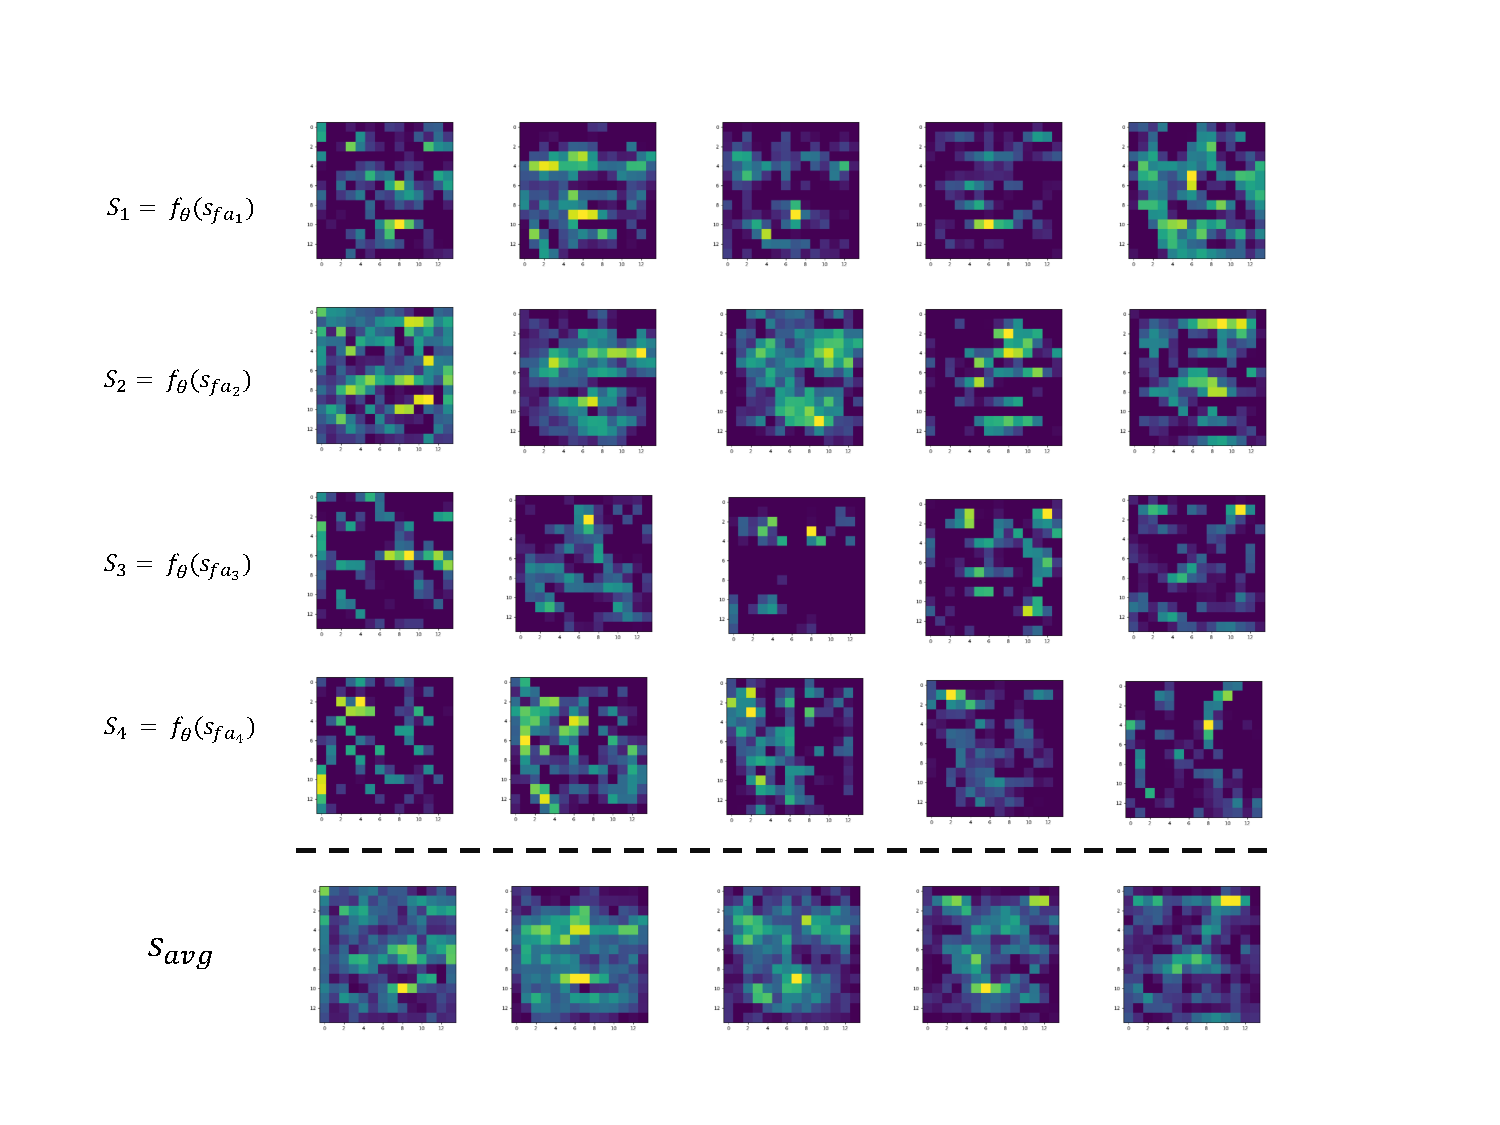
\includegraphics[width=\textwidth]{fig/feature_compare.pdf}
\caption{Visual comparison between U-Net intermediate features 
modulated by the high-frequency band $\mathcal{H}$ at the 
decoder, the low-frequency band $\mathcal{L}$ at the encoder, 
and the unmodulated baseline features. Important textural 
details are highlighted in brighter colors.}
\label{fig:feature_compare}
\end{sidewaysfigure}

Examining the high-frequency band features at 
\texttt{up\_blocks[1]}, it is apparent that fine textural 
details such as edges, textures, and high-frequency patterns 
are highlighted in brighter colors. Also, it is possible to 
recognize sharp boundary structures and high-contrast 
patterns. However, when observing the low-frequency band 
features at \texttt{down\_blocks[1]}, it is evident that the 
coarse structural patterns are emphasized while the fine 
textural details are diminished. Conversely, the unmodulated 
baseline features capture neither the fine textural details 
nor the coarse structural patterns prominently, leading to 
over-smoothed outputs that lack both perceptual sharpness and 
structural clarity.

The single-injection design has limitations as it keeps losing 
important information from one frequency band while 
over-emphasizing the other. On the other hand, the BD-SFT 
overcomes this limitation by selectively injecting both 
frequency bands at functionally distinct U-Net stages, 
preserving fine textural details at the decoder while 
avoiding any degradation of coarse structural patterns at the 
encoder. To verify this claim quantitatively, three variants 
are evaluated by selectively disabling SFT modulation at 
inference time. The \textit{w/o HIGH} variant disables the 
high-frequency injection at the decoder by setting 
$\gamma_{\mathcal{H}} = 1$ and $\beta_{\mathcal{H}} = 0$ 
(identity modulation). The \textit{w/o LOW} variant disables 
the low-frequency injection at the encoder by setting 
$\gamma_{\mathcal{L}} = 1$ and $\beta_{\mathcal{L}} = 0$. The 
\textit{w/o both} variant disables both injections, reducing 
the framework to the StableVSR baseline behavior. The same 
trained model is used for all variants; only the 
inference-time SFT modulation is selectively disabled. This 
isolates the contribution of each band without confounding 
the effects of independent training trajectories.

\begin{table}[htbp]
\caption{Ablation study on frequency band injection (REDS4).}
\centering
\resizebox{\textwidth}{!}{
\begin{tabular}{|l|c|c|c|c|c|c|c|c|c|}
\hline
Variant & PSNR$\uparrow$ & SSIM$\uparrow$ & LPIPS$\downarrow$ & 
DISTS$\downarrow$ & MUSIQ$\uparrow$ & CLIP-IQA$\uparrow$ & 
NIQE$\downarrow$ & tLPIPS$\downarrow$ & tOF$\downarrow$ \\ 
\hline\hline
WC-BD-SFT (full) 
& 24.48 & \textbf{0.691} & \textbf{0.193} & \textbf{0.088} 
& \textbf{65.70} & \textbf{0.386} & \textbf{2.77} 
& \textbf{15.25} & \textbf{11.120} \\
w/o HIGH & XX.XX & X.XXX & X.XXX & X.XXX & 64.49 & X.XXX 
& X.XX & 22.11 & XX.XXX \\
w/o LOW & \textbf{24.70} & X.XXX & X.XXX & X.XXX & 63.39 
& 0.335 & X.XX & 16.57 & XX.XXX \\
w/o both & XX.XX & X.XXX & 0.247 & X.XXX & 59.35 & X.XXX 
& X.XX & 25.18 & XX.XXX \\
\hline
\end{tabular}}
\label{tab:ablation_band}
\end{table}

Table~\ref{tab:ablation_band} confirms the visual observations 
quantitatively. Disabling high-frequency injection 
(\textit{w/o HIGH}) increases tLPIPS from 15.25 to 22.11 
($+45.0\%$), validating that the high-frequency band, injected 
at the decoder where textural details are synthesized, plays 
the dominant role in stabilizing inter-frame texture coherence. 
Disabling low-frequency injection (\textit{w/o LOW}) causes 
MUSIQ to drop from 65.70 to 63.39 and CLIP-IQA from 0.386 to 
0.335, while PSNR slightly increases to 24.70, suggesting that 
low-frequency conditioning at the encoder shapes the 
structural representation in a way that improves perceptual 
naturalness at the cost of pixel-level fidelity. When both 
injections are disabled (\textit{w/o both}), LPIPS increases 
to 0.247, exceeding the sum of degradations from disabling 
each band individually, indicating that the two bands carry 
complementary information that interacts non-linearly within 
the U-Net.


\subsection{Ablation study on the impact of magnitude-phase 
decoupled processing in SubbandBlock}
\label{subsec:ablation_magphase}

The SubbandBlock processes the magnitude and phase components 
of the DT-CWT coefficients separately through dedicated 
parallel branches before recombining them into the final 
conditioning features. Both branches apply the same operator 
$\mathcal{E}(\cdot) = \mathrm{Conv}_{1\times1} \circ 
\mathrm{SA} \circ \mathrm{SiLU} \circ \mathrm{DWConv}_{3\times3}$ 
before recombination. The reason for performing the decoupled 
processing is as follows.

The magnitude component contains the energy distribution of 
each directional subband, characterized by non-negative values 
and near shift-invariance properties. On the other hand, the 
phase component encodes precise spatial localization within 
the subband, characterized by $2\pi$-periodic values with 
discontinuity at the wraparound boundary. In this way, 
processing both components through a single shared branch may 
force the network to mix these two fundamentally different 
signals at the first convolutional layer, potentially diluting 
their distinct contributions. Motivated by this observation, 
we adopt parallel branches with recombination.

\begin{table}[b]
\caption{Performance comparison based on the SubbandBlock's 
magnitude-phase processing strategy on REDS4.}
\centering
\resizebox{\textwidth}{!}{
\begin{tabular}{|l|l|c|c|c|c|}
\hline
Dataset & Method & LPIPS$\downarrow$ & MUSIQ$\uparrow$ & 
tLPIPS$\downarrow$ & Mean rank \\ 
\hline\hline
REDS4 & StableVSR                       & 0.309 & 42.79 & 41.11 & 4.0 \\
      & WC-BD-SFT + Joint Mag-Phase     & X.XXX & XX.XX & XX.XX & X.X \\
      & WC-BD-SFT + Decoupled (Ours)    & \textbf{0.193} & \textbf{65.70} & \textbf{15.25} & \textbf{1.0} \\ 
\hline
\end{tabular}}
\label{tab:ablation_magphase}
\end{table}

To compare the two strategies, we conducted experiments on the 
joint variant where magnitude $M^{(j)}$ (18 channels) and 
trigonometric phase encoding $\mathcal{T}(\phi^{(j)}) = 
(\sin\phi^{(j)}, \cos\phi^{(j)})$ (36 channels) are 
concatenated along the channel dimension to form a single 
tensor of $54$ channels, processed through a single shared 
branch with the same operator $\mathcal{E}(\cdot)$, then 
directly fed to the SFT heads without recombination. The two 
variants share the same training configuration, total 
parameter budget, and frequency band partitioning, so the 
comparison isolates the effect of the decoupled-versus-joint 
processing strategy.

The performance result is shown in 
Table~\ref{tab:ablation_magphase}. Decoupled magnitude-phase 
processing outperforms joint processing on both perceptual 
quality (LPIPS, MUSIQ) and temporal consistency (tLPIPS), 
supporting the use of parallel branches with recombination.


\subsection{Ablation study on fine-tuning weights on individual 
loss components}
\label{subsec:ablation_loss_weights}

In this section, we conduct experiments by tuning the lambda 
values for each loss component while varying their proportions 
to investigate how the weight ratio affects the perceptual 
quality.

We investigate the influence of the three loss components 
(high-frequency band $\mathcal{H}$, low-frequency band 
$\mathcal{L}$, and lowpass band) by varying their lambda 
values from $0.1$ to $1.0$. Additionally, we test a uniform 
weight ratio of $1.0{:}1.0{:}1.0$ for all three components 
to see how it compares with the proposed setting.

The experiments were conducted using the REDS4 in-domain 
evaluation set. The average results represent the performance 
obtained by training the model on the REDS training split for 
20{,}000 iterations and then testing it on the four reserved 
REDS4 sequences (clip indices 000, 011, 015, 020). According 
to the results presented in 
Table~\ref{tab:additional_lambda1}, the proposed weight ratio 
of $0.1{:}1.0{:}1.0$ yielded the best perceptual quality.

\begin{table}[t]
\caption{The comparison of perceptual quality on REDS4 in 
different weights on individual loss components.}
\centering
\resizebox{\textwidth}{!}{
\begin{tabular}{|l|l|c|c|c|c|}
\hline
\multirow{2}{*}{Dataset} & \multirow{2}{*}{Method} & 
\multicolumn{3}{c|}{Weights on each loss component} & 
\multirow{2}{*}{\begin{tabular}[c]{@{}c@{}}LPIPS$\downarrow$ /\\ tLPIPS$\downarrow$\end{tabular}} \\ 
\cline{3-5}
& & $\lambda_{\mathcal{H}}$ & $\lambda_{\mathcal{L}}$ & 
$\lambda_{\mathrm{LP}}$ & \\ 
\hline\hline
\multirow{4}{*}{REDS4} & WC-BD-SFT 
& 0.1 & 0.5 & 0.5 & X.XXX / XX.XX \\ \cline{3-6}
& & 0.5 & 0.5 & 0.5 & X.XXX / XX.XX \\ \cline{3-6}
& & 1.0 & 1.0 & 1.0 & X.XXX / XX.XX \\ \cline{3-6}
& & 0.1 & 1.0 & 1.0 & \textbf{0.193 / 15.25} \\ 
\hline
\end{tabular}}
\label{tab:additional_lambda1}
\end{table}

We observed that when the high-frequency loss component was 
given a smaller weight $\lambda_{\mathcal{H}} = 0.1$ relative 
to the low-frequency and lowpass components, the perceptual 
quality reached LPIPS $0.193$ and tLPIPS $15.25$. Therefore, 
we conducted further experiments by gradually decreasing the 
weight on the high-frequency component (from $0.1$ down to 
$0.0$) while keeping the rest of the components at $1.0$ to 
explore whether further reduction would lead to better 
performance. As shown in Table~\ref{tab:additional_lambda2}, 
none of these settings surpassed the best performance of 
LPIPS $0.193$ and tLPIPS $15.25$.

\begin{table}[b]
\caption{The comparison of perceptual quality on REDS4 with 
various combinations of weights on each individual loss 
component.}
\centering
\resizebox{\textwidth}{!}{
\begin{tabular}{|l|l|c|c|c|c|}
\hline
\multirow{2}{*}{Dataset} & \multirow{2}{*}{Method} & 
\multicolumn{3}{c|}{Weights on each loss component} & 
\multirow{2}{*}{\begin{tabular}[c]{@{}c@{}}LPIPS$\downarrow$ /\\ tLPIPS$\downarrow$\end{tabular}} \\ 
\cline{3-5}
& & $\lambda_{\mathcal{H}}$ & $\lambda_{\mathcal{L}}$ & 
$\lambda_{\mathrm{LP}}$ & \\ 
\hline\hline
\multirow{4}{*}{REDS4} & WC-BD-SFT 
& 0.05 & 1.0 & 1.0 & X.XXX / XX.XX \\ \cline{3-6}
& & 0.01 & 1.0 & 1.0 & X.XXX / XX.XX \\ \cline{3-6}
& & 0.0 & 1.0 & 1.0 & X.XXX / XX.XX \\ \cline{3-6}
& & 0.1 & 1.0 & 1.0 & \textbf{0.193 / 15.25} \\ 
\hline
\end{tabular}}
\label{tab:additional_lambda2}
\end{table}

These results support the design intent that the 
high-frequency band serves as a soft texture prior requiring 
only a small relative weight, while the low-frequency and 
lowpass components require strong supervision for structural 
reconstruction. Maintaining the smaller weight on the 
high-frequency component while keeping the same weight ratio 
for the low-frequency and lowpass components resulted in the 
best perceptual quality.


%==================== Section =====================%
\section{Qualitative Results}
\label{sec:qualitative}

This section presents qualitative comparisons that complement 
the quantitative analysis. While quantitative metrics summarize 
performance into single numbers, visual comparisons reveal 
aspects of perceptual quality and temporal consistency that 
are difficult to capture numerically. Three types of 
visualizations are provided: single-frame comparisons on the 
in-domain REDS4 set, single-frame comparisons across the three 
cross-dataset benchmarks, and temporal consistency comparisons 
that visualize inter-frame behavior.


\subsection{Single-Frame Comparison on REDS4}
\label{subsec:qualitative_reds4}

Figure~\ref{fig:qualitative_reds4} shows visual comparisons on 
representative frames from the REDS4 evaluation set. For each 
example, the bicubic-upsampled low-resolution input, the 
outputs of BasicVSR++ \cite{chan2022basicvsrplusplus} and 
StableVSR \cite{rota2024stablevsr}, the proposed method, and 
the ground truth are shown side by side. Zoomed-in patches 
highlight regions with fine textural details, sharp edges, 
and high-frequency patterns that are particularly challenging 
for super-resolution methods.

\begin{sidewaysfigure}
\centering
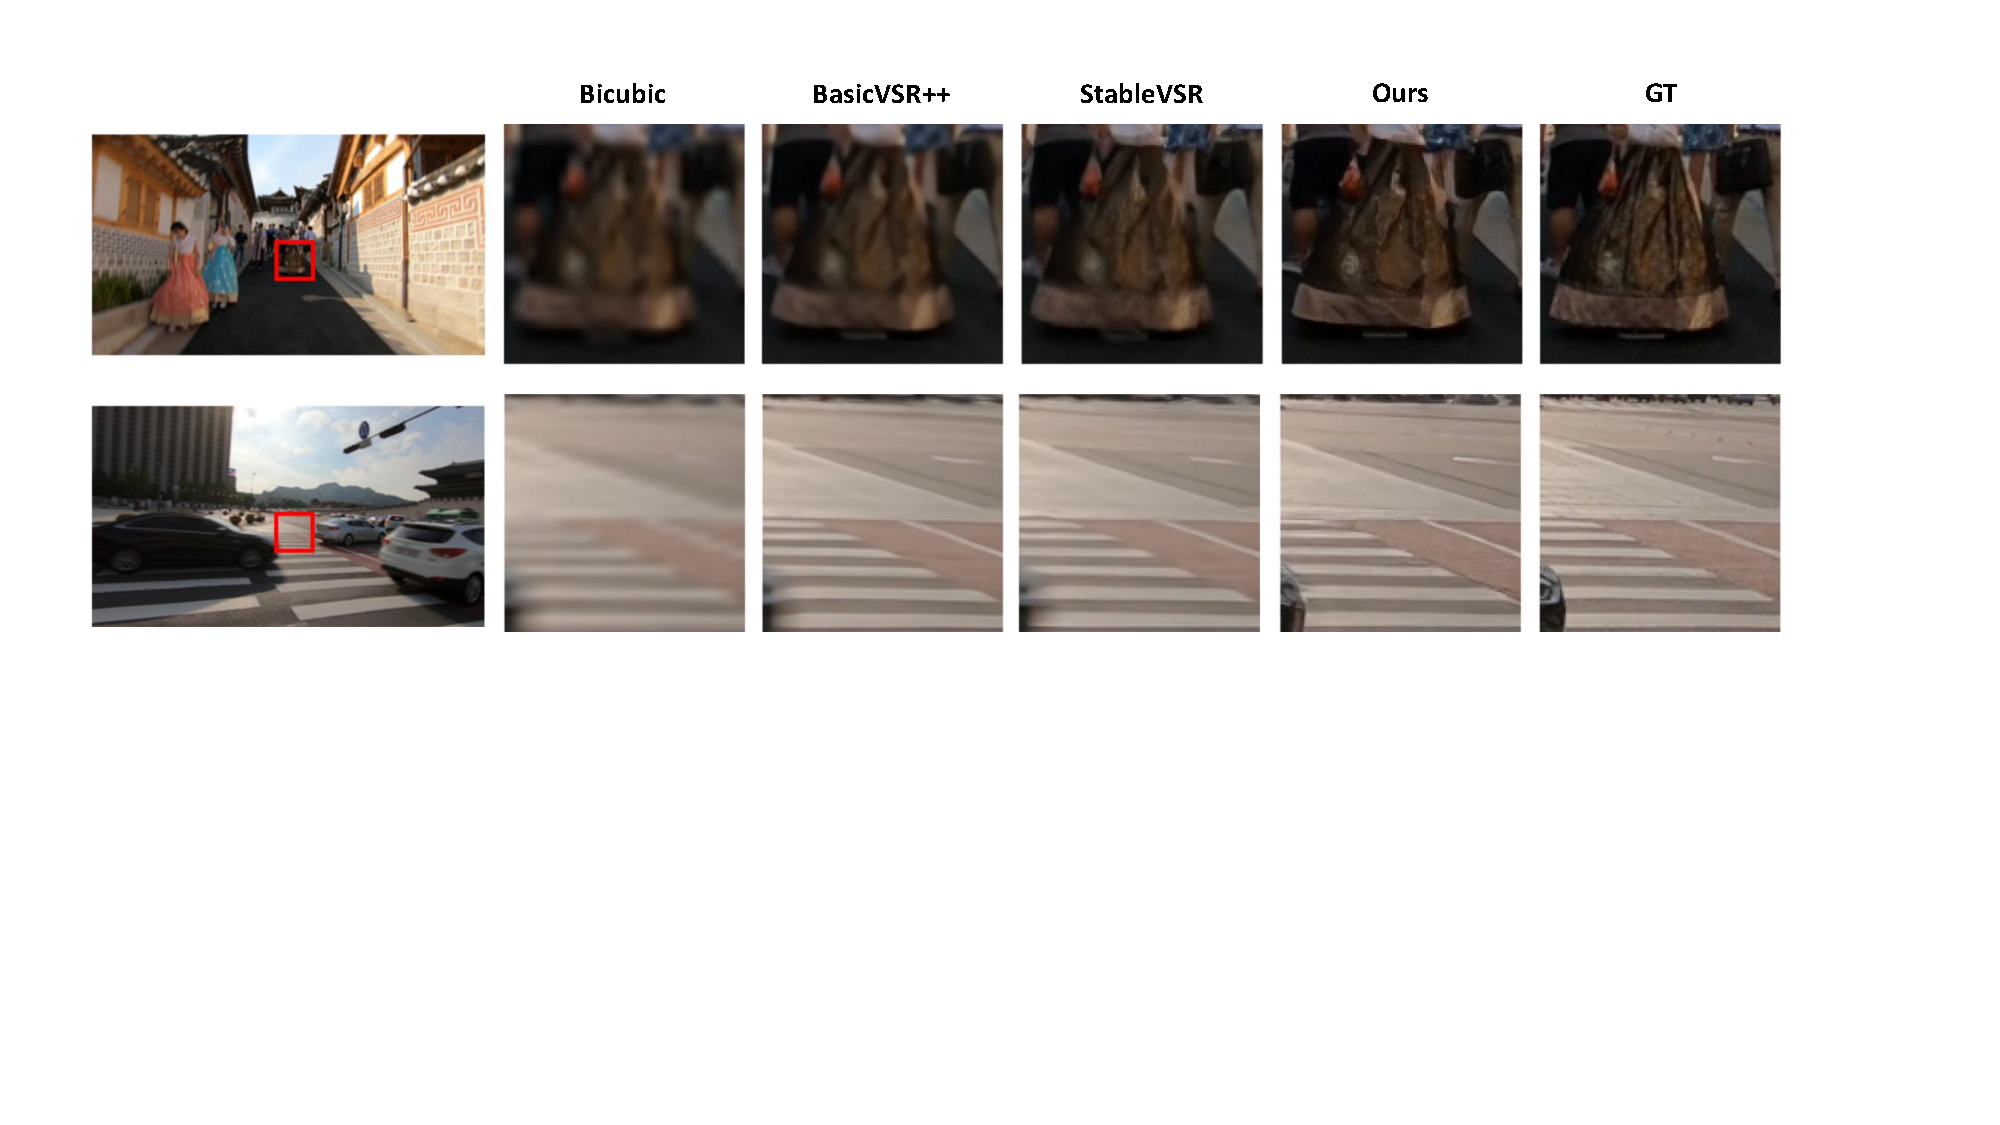
\includegraphics[width=\textheight,trim={0 250 0 0},clip]{fig/qualitative_reds4.pdf}
\caption{Qualitative comparison on REDS4. From left to right: 
bicubic upsampling, BasicVSR++ \cite{chan2022basicvsrplusplus}, 
StableVSR \cite{rota2024stablevsr}, the proposed method, and 
the ground-truth high-resolution frame. Zoomed-in patches 
highlight fine details. The proposed method recovers sharper 
textures and finer details compared to both baselines, while 
remaining faithful to the ground-truth structure.}
\label{fig:qualitative_reds4}
\end{sidewaysfigure}

The visual comparison reveals three observations. First, 
BasicVSR++ produces outputs that are over-smoothed and lack 
high-frequency details, consistent with its higher PSNR but 
lower perceptual scores. Second, StableVSR generates more 
realistic textures than BasicVSR++ but exhibits noticeable 
artifacts in fine-detail regions, where the diffusion process 
can introduce unrealistic patterns. Third, the proposed method 
produces sharper and more natural textures compared to both 
baselines, with clearer edge definition and finer texture 
detail. This is particularly evident in regions containing 
text, repeated patterns, and high-contrast structures, where 
the frequency-domain conditioning provides explicit guidance 
that complements the spatial-domain ControlNet branch.


\subsection{Cross-Dataset Visual Comparison}
\label{subsec:qualitative_cross}

Figure~\ref{fig:qualitative_cross} presents qualitative 
comparisons on the three cross-dataset benchmarks: Vid4 
\cite{liu2013vid4}, UDM10 \cite{yi2019udm10}, and SPMCS 
\cite{tao2017spmcs}. These datasets contain content unseen 
during training, providing a stringent test of generalization 
capability.

\begin{sidewaysfigure}
\centering
\includegraphics[width=\textheight,trim={0 250 0 0},clip]{fig/qualitative_cross.pdf}
\caption{Qualitative comparison across cross-dataset 
benchmarks. Top row: Vid4 (calendar). Middle row: UDM10 
(architectural structure). Bottom row: SPMCS (outdoor scene). 
For each row, columns show: bicubic upsampling, BasicVSR++ 
\cite{chan2022basicvsrplusplus}, StableVSR 
\cite{rota2024stablevsr}, the proposed method, and the 
ground-truth high-resolution frame.}
\label{fig:qualitative_cross}
\end{sidewaysfigure}

The cross-dataset comparison confirms that the visual quality 
improvements observed on REDS4 generalize to unseen content. 
On Vid4's calendar sequence, where text legibility is the 
primary challenge, the proposed method recovers sharper 
character boundaries compared to StableVSR. On UDM10, which 
contains architectural structures with strong directional 
patterns, the proposed method preserves edge orientation more 
accurately, benefiting from the directional selectivity of 
DT-CWT coefficients. On SPMCS, which contains the most diverse 
content including outdoor scenes with complex textures, the 
proposed method maintains realistic texture appearance without 
the flickering artifacts visible in StableVSR's output.


\subsection{Frequency-Domain Analysis}
\label{subsec:qualitative_frequency}

To validate the contribution of the proposed wavelet-based 
conditioning, we analyze the frequency-domain characteristics 
of the super-resolved outputs by computing the radial power 
spectrum ratio relative to the ground truth across spatial 
frequency bands.

\begin{figure}[H]
\centering
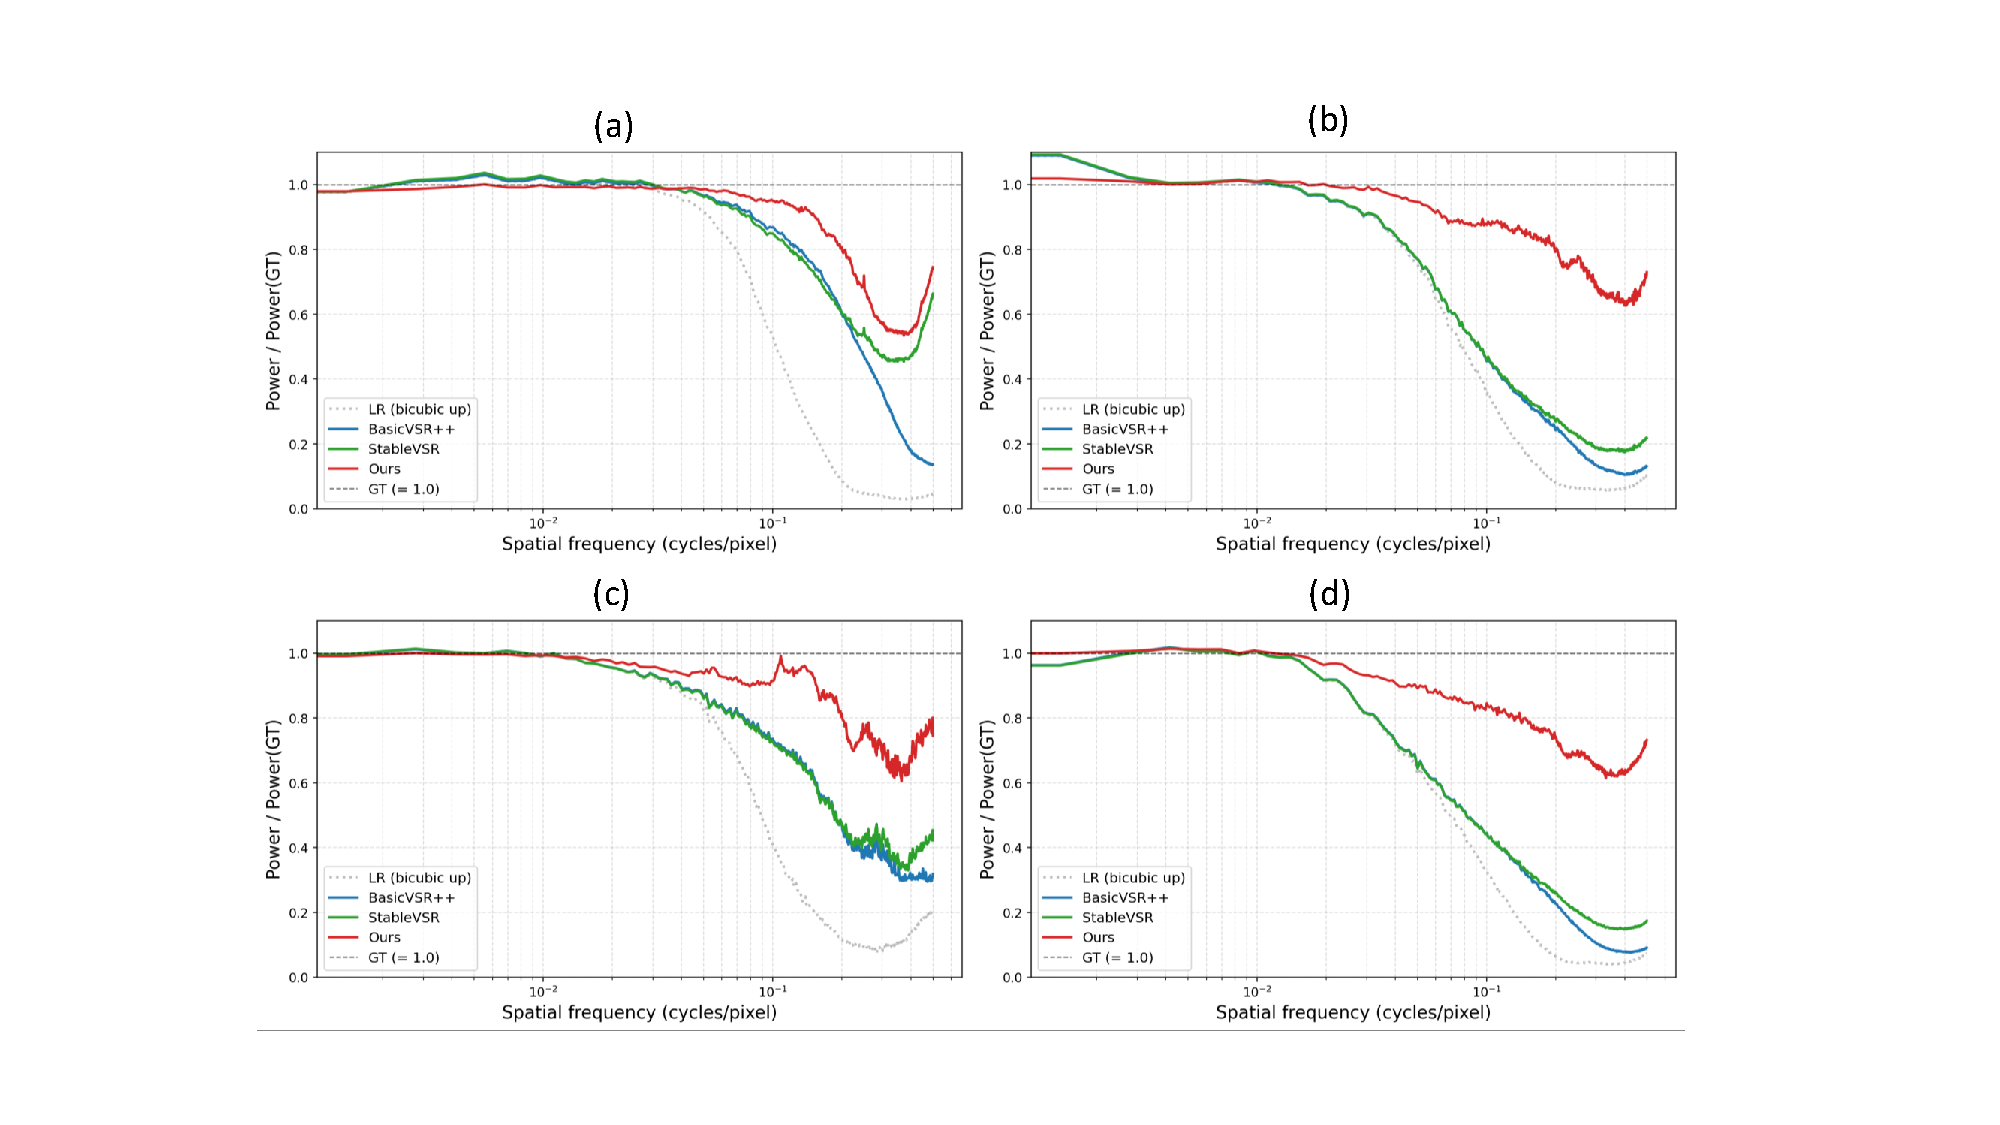
\includegraphics[width=\textwidth]{fig/radial_spectrum_reds4.pdf}
\caption{Radial power spectrum ratio to ground truth on the 
four REDS4 sequences (000, 011, 015, 020). The horizontal 
axis represents normalized spatial frequency in cycles per 
pixel (log scale), and the vertical axis represents the ratio 
of each method's power spectrum to that of the ground-truth 
high-resolution video. A ratio of $1.0$ (gray dashed line) 
indicates perfect spectral matching with the ground truth.}
\label{fig:radial_spectrum}
\end{figure}

Figure~\ref{fig:radial_spectrum} reveals three findings 
consistent across all four REDS4 sequences. First, at low 
frequencies, all methods including the LR bicubic upsampling 
closely match the ground truth, indicating that low-frequency 
structures are well-recovered by all approaches. Second, at 
mid frequencies, substantial differences emerge: BasicVSR++ 
and StableVSR exhibit rapid attenuation, while the proposed 
method maintains ratios close to the ground truth. Third, at 
high frequencies, the gap is most pronounced. BasicVSR++ and 
StableVSR exhibit power ratios of approximately $0.10$--$0.45$ 
at $f \approx 0.3$, while the proposed method maintains 
ratios of $0.55$--$0.65$.

To quantify these observations, Table~\ref{tab:freq_band} 
reports the mean power ratio averaged over the four REDS4 
sequences and 100 frames per sequence, partitioned into three 
frequency bands: low ($f \in [0, 0.05]$), mid 
($f \in [0.05, 0.15]$), and high ($f \in [0.15, 0.5]$).

\begin{table}[h]
\centering
\caption{Frequency-band power ratio to ground truth on REDS4 
(averaged over four sequences $\times$ 100 frames). Values 
closer to GT (= 1.0) indicate better spectral matching. 
Best results in bold.}
\label{tab:freq_band}
\begin{tabular}{|l|c|c|c|}
\hline
Method & Low ($0$--$0.05$) & Mid ($0.05$--$0.15$) & 
High ($0.15$--$0.5$) \\
\hline\hline
LR (bicubic up) & 0.929 & 0.441 & 0.080 \\
BasicVSR++ \cite{chan2022basicvsrplusplus} & 0.937 & 0.639 & 0.255 \\
StableVSR \cite{rota2024stablevsr} & 0.938 & 0.635 & 0.341 \\
Ours & \textbf{0.975} & \textbf{0.900} & \textbf{0.693} \\
\hline
\end{tabular}
\end{table}

Table~\ref{tab:freq_band} confirms the visual observations 
quantitatively. In the low-frequency band, all methods 
recover $\geq 92\%$ of the ground-truth power, indicating 
that low-frequency structures are well-preserved across all 
approaches. In the mid-frequency band, the proposed method 
achieves $0.900$, substantially higher than BasicVSR++ 
($0.639$) and StableVSR ($0.635$), representing a $+41.7\%$ 
relative improvement over StableVSR. In the high-frequency 
band, where the texture detail synthesis matters most, the 
proposed method achieves $0.693$ versus StableVSR's $0.341$, 
representing a $+103.2\%$ relative improvement, more than 
doubling the high-frequency power retention.

This frequency-domain perspective directly validates the core 
hypothesis underlying the proposed method: by routing DT-CWT 
high-frequency band coefficients to the U-Net decoder and 
low-frequency band coefficients to the encoder, the framework 
leverages frequency-aware conditioning to preserve the 
spectral content that pixel-level losses fail to enforce. 
Notably, the gap between BasicVSR++ and StableVSR in the 
mid-frequency band is small ($0.639$ vs.\ $0.635$), 
suggesting that the diffusion prior alone provides limited 
benefit for mid-frequency texture recovery. The substantial 
improvement of the proposed method over StableVSR ($0.900$ 
vs.\ $0.635$ in mid-band, $0.693$ vs.\ $0.341$ in high-band) 
isolates the contribution of the wavelet-conditioned BD-SFT 
modulation, since both methods share the same diffusion 
backbone (Stable Diffusion v2.1) and ControlNet conditioning.


\subsection{Temporal Consistency Visualization}
\label{subsec:qualitative_temporal}

To visualize temporal behavior, we extract a horizontal 
scanline at a fixed $y$-coordinate from each generated frame 
and stack them along the time axis. This produces a 2D image 
where the horizontal axis represents spatial position and the 
vertical axis represents time. In this representation, smooth 
horizontal stripes indicate that the same texture is 
consistently rendered across consecutive frames, while noisy 
or discontinuous patterns indicate temporal flickering.

\begin{figure}[h]
\centering
\includegraphics[width=\textwidth]{fig/temporal_profile.pdf}
\caption{Temporal profile comparison on a REDS4 sequence. A 
horizontal scanline at a fixed $y$-coordinate is extracted 
from each frame and stacked along the time axis. From left 
to right: BasicVSR++ \cite{chan2022basicvsrplusplus}, 
StableVSR \cite{rota2024stablevsr}, the proposed method, and 
the ground-truth high-resolution video. Smooth horizontal 
stripes indicate temporally consistent textures, while noisy 
or discontinuous patterns indicate flickering. The proposed 
method produces profiles that closely match the ground truth, 
while StableVSR exhibits visible flickering artifacts.}
\label{fig:temporal_profile}
\end{figure}

The temporal profile in Figure~\ref{fig:temporal_profile} 
provides direct visual evidence for the substantial reduction 
in tLPIPS reported in Table~\ref{tab:accuracy_reds4} 
($41.11 \to 15.25$, a $62.9\%$ reduction). The StableVSR 
profile exhibits visible noise patterns and inconsistent 
texture rendering across the time axis, reflecting the texture 
flickering issue characteristic of diffusion-based VSR methods 
due to the stochastic nature of the denoising process. In 
contrast, the profile from the proposed method exhibits 
smoother stripes that closely match the ground-truth profile, 
demonstrating that the band-decoupled wavelet conditioning 
effectively stabilizes the generative process across 
consecutive frames. BasicVSR++ also produces smooth profiles 
due to its deterministic feed-forward nature but lacks 
high-frequency texture detail compared to the proposed method 
and the ground truth.

This temporal-domain perspective complements the standard 
temporal metric (tLPIPS) by directly visualizing the stability 
of texture rendering over time, producing temporally coherent 
textures suitable for video applications.